\documentclass[journal]{IEEEtran}

\usepackage{amsmath,amssymb,amsthm}
\usepackage{booktabs}
\usepackage{array}
\usepackage{graphicx}
\usepackage{pgfplots}
\usepgfplotslibrary{groupplots}
\pgfplotsset{compat=1.18}
\usepackage{cite}
\usepackage{url}
\usepackage[hidelinks]{hyperref}
\usepackage{microtype}
\usepackage{docmute}
\usepackage{etoolbox}

\newtheorem{theorem}{Theorem}
\newtheorem{corollary}{Corollary}
\newtheorem{proposition}{Proposition}
\newtheorem{remark}{Remark}

\newcommand{\Pone}{\mathbb{P}_1}
\newcommand{\Pzero}{\mathbb{P}_0}
\newcommand{\Eone}{\mathbb{E}_1}
\newcommand{\Ezero}{\mathbb{E}_0}
\newcommand{\LR}{\Lambda}
\newcommand{\ind}{\mathbf{1}}

\title{Boundary-Localized Genomic Utility and Clinical-Tail Dominance:\\
A Likelihood-Ratio Theory for ZeBRA and Fibrotic Interstitial Lung Disease}
\author{Ishanu Chattopadhyay\\
Division of Biomedical Informatics, University of Kentucky College of Medicine}

\newcommand{\empiricalcallout}{%
\par\noindent
The current Colorado analysis is summarized in Section~\ref{sec:empirical}. The central empirical distinction is between \emph{global incremental discrimination}, for which broad genomic augmentation provides no meaningful gain over ZeBRA, and \emph{localized decision utility}, for which \textit{MUC5B} retains conditional information within restricted ZeBRA operating regions.
\par
}

\newcommand{\empiricalsection}{%
\origsection{Empirical correspondence in the Colorado ILD analysis}
\label{sec:empirical}

\subsection{Cohort and analysis geometry}

The current analysis uses the Colorado genomic--clinical cohort assembled in \texttt{zebra\_comp}. Three stored phenotype fields are evaluated: \texttt{FILD or FILA ADJUDICATED}, \texttt{NONFIBROTIC ILD ADJUDICATED}, and \texttt{NON FIBROTIC ILA ADJUDICATED}. The operational target construction maps \texttt{Y/y} to 1 and \texttt{N/n} to 0, converts the field to numeric, assigns missing target values to 0, and excludes observations without an available 104-week ZeBRA score. Thus the reported endpoint is the notebook-defined prediction target; not every target-zero observation is an independently adjudicated negative. This distinction is especially important when interpreting false-positive rates.

The processed genomic matrix contains 171 selected variant loci represented by categorical genotype states; rs35705950 in \textit{MUC5B} is included explicitly. The principal global comparison uses 30 repeated stratified outer splits with 40\% training and 60\% held-out evaluation. Within each split, ZeBRA is evaluated as the existing clinical-history score, a genomic-only LightGBM model is fitted to the genomic variables, and a combined LightGBM model is fitted to genomics plus ZeBRA.

\subsection{Global discrimination: clinical history dominates}

Across 30 repeated held-out splits, ZeBRA was the strongest predictor for all three endpoints. For FILD/FILA, mean AUC was 0.8142 for ZeBRA, 0.5662 for genomics alone, and 0.7988 for the nonlinear combined model. The same ordering was more pronounced for the two nonfibrotic outcomes (Table~\ref{tab:auc-repeated}; Fig.~\ref{fig:global-auc}). These repeated-split results supersede the earlier single-split comparison as the primary global-discrimination analysis.

\begin{table*}[!t]
\caption{Held-out AUC over 30 repeated outer splits. Values are mean $\pm$ SD.}
\label{tab:auc-repeated}
\centering
\footnotesize
\setlength{\tabcolsep}{8pt}
\begin{tabular}{lccc}
\toprule
Target & ZeBRA & Genomic & Combined\\
\midrule
FILD/FILA & $0.8142\pm0.0089$ & $0.5662\pm0.0245$ & $0.7988\pm0.0150$\\
Nonfibrotic ILD & $0.8202\pm0.0257$ & $0.5141\pm0.0719$ & $0.6145\pm0.0953$\\
Nonfibrotic ILA & $0.8281\pm0.0162$ & $0.4717\pm0.0443$ & $0.7112\pm0.0541$\\
\bottomrule
\end{tabular}
\end{table*}

\begin{figure*}[!t]
\centering
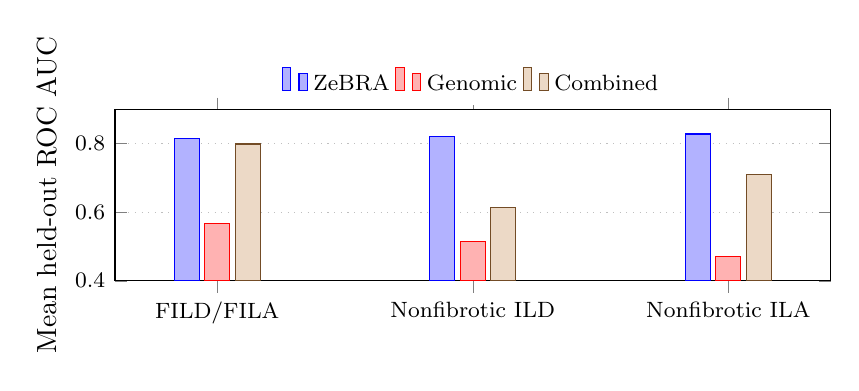
\begin{tikzpicture}
\begin{axis}[
width=0.88\textwidth,height=0.31\textwidth,
ybar,bar width=9pt,
ymin=0.40,ymax=0.90,
ylabel={Mean held-out ROC AUC},
symbolic x coords={FILD/FILA,Nonfibrotic ILD,Nonfibrotic ILA},
xtick=data,
xticklabel style={font=\footnotesize},
yticklabel style={font=\footnotesize},
legend style={at={(0.5,1.02)},anchor=south,legend columns=3,draw=none,font=\footnotesize},
major grid style={dotted},ymajorgrids=true,
enlarge x limits=0.20]
\addplot coordinates {(FILD/FILA,0.8142) (Nonfibrotic ILD,0.8202) (Nonfibrotic ILA,0.8281)};
\addlegendentry{ZeBRA}
\addplot coordinates {(FILD/FILA,0.5662) (Nonfibrotic ILD,0.5141) (Nonfibrotic ILA,0.4717)};
\addlegendentry{Genomic}
\addplot coordinates {(FILD/FILA,0.7988) (Nonfibrotic ILD,0.6145) (Nonfibrotic ILA,0.7112)};
\addlegendentry{Combined}
\end{axis}
\end{tikzpicture}
\caption{Global discrimination across three phenotype targets. Bars show mean held-out AUC over 30 repeated outer splits. Genomics alone is substantially weaker than ZeBRA, and indiscriminate global combination does not improve the clinical-history predictor.}
\label{fig:global-auc}
\end{figure*}

The marginal AUC distributions overlap for ZeBRA and the combined model in FILD/FILA, but overlap of boxplots is not a statistical test because the models share the same repeated splits. More importantly, the scientific question is whether genomic information yields a reproducible \emph{incremental gain} once ZeBRA is known. We therefore performed a second explicitly paired analysis.

\subsection{Paired incremental value is essentially zero for FILD/FILA}

A separate 30-split analysis compared a ZeBRA-only logistic model with a regularized elastic-net model containing ZeBRA plus the complete genomic panel on the same held-out subjects in each split. For FILD/FILA, mean AUC was 0.81250 for ZeBRA and 0.81293 for ZeBRA plus genomics. The paired mean difference was only $+0.00043$, the median difference was 0, and the split-wise 2.5th--97.5th percentile range was $[-0.00507,0.00408]$ (Fig.~\ref{fig:incremental-auc}). Thus the data do not support a meaningful global FILD/FILA AUC improvement from broad genomic augmentation.

Proper scoring rules reinforce this conclusion. For FILD/FILA, adding all genomic variables decreased average precision by 0.0311 on average and worsened Brier score and log loss in all 30 splits (mean $\Delta$Brier $=+3.12\times10^{-4}$; mean $\Delta$log-loss $=+0.00468$, where positive differences are worse). For nonfibrotic ILD and ILA, mean paired AUC changes were -0.1005 and -0.0374, respectively.

\begin{figure*}[!t]
\centering
\begin{tikzpicture}
\begin{axis}[
width=0.82\textwidth,height=0.29\textwidth,
xmin=0.5,xmax=3.5,
ymin=-0.24,ymax=0.03,
xtick={1,2,3},xticklabels={FILD/FILA,Nonfibrotic ILD,Nonfibrotic ILA},
ylabel={Paired $\Delta$AUC (genomics + ZeBRA $-$ ZeBRA)},
tick label style={font=\footnotesize},label style={font=\footnotesize},
ymajorgrids=true,major grid style={dotted}]
\addplot+[only marks,mark=*] coordinates {(1,0.00043) (2,-0.10052) (3,-0.03737)};
\addplot+[no marks,dashed] coordinates {(0.5,0) (3.5,0)};
\draw (axis cs:1,-0.00507) -- (axis cs:1,0.00408);
\draw (axis cs:0.94,-0.00507) -- (axis cs:1.06,-0.00507);
\draw (axis cs:0.94,0.00408) -- (axis cs:1.06,0.00408);
\draw (axis cs:2,-0.22577) -- (axis cs:2,-0.00506);
\draw (axis cs:1.94,-0.22577) -- (axis cs:2.06,-0.22577);
\draw (axis cs:1.94,-0.00506) -- (axis cs:2.06,-0.00506);
\draw (axis cs:3,-0.07384) -- (axis cs:3,-0.00705);
\draw (axis cs:2.94,-0.07384) -- (axis cs:3.06,-0.07384);
\draw (axis cs:2.94,-0.00705) -- (axis cs:3.06,-0.00705);
\end{axis}
\end{tikzpicture}
\caption{Paired incremental AUC from the regularized analysis. Points are mean paired differences; vertical intervals show the split-wise 2.5th--97.5th percentile range. FILD/FILA is centered essentially at zero, while the two nonfibrotic endpoints worsen with global genomic augmentation.}
\label{fig:incremental-auc}
\end{figure*}

\subsection{ZeBRA does not reconstruct \textit{MUC5B} genotype}

A possible explanation for weak global genomic increment is that the clinical history has already reconstructed the major genetic signal. The data do not support that interpretation. Among 12,766 subjects with a called rs35705950 genotype, 2,499 were \textit{MUC5B} T-allele carriers (19.6\%). ZeBRA predicted carrier status at essentially chance level: raw AUC 0.5088, five-fold cross-validated linear-logistic AUC 0.5040, spline-logistic AUC 0.5021, Pearson $r=0.0107$ ($p=0.228$), and Spearman $\rho=0.0120$ ($p=0.174$).

There was nevertheless an apparent pooled tail association: the top 1\% of the ZeBRA distribution showed 1.47-fold \textit{MUC5B} carrier enrichment, with permutation-adjusted $p\approx0.009$. That concordance disappears after conditioning on FILD/FILA status. Among explicitly adjudicated FILD/FILA-negative subjects, the continuous ZeBRA-to-carrier AUC was 0.485; among FILD/FILA-positive subjects it was 0.482. In contrast, carrier prevalence was 39.3\% among FILD/FILA-positive subjects compared with 19.2\% among explicitly adjudicated negatives (Fig.~\ref{fig:muc5b-strata}). The pooled signal is therefore consistent with both ZeBRA and \textit{MUC5B} tracking disease, rather than ZeBRA encoding genotype.

\begin{figure*}[!t]
\centering
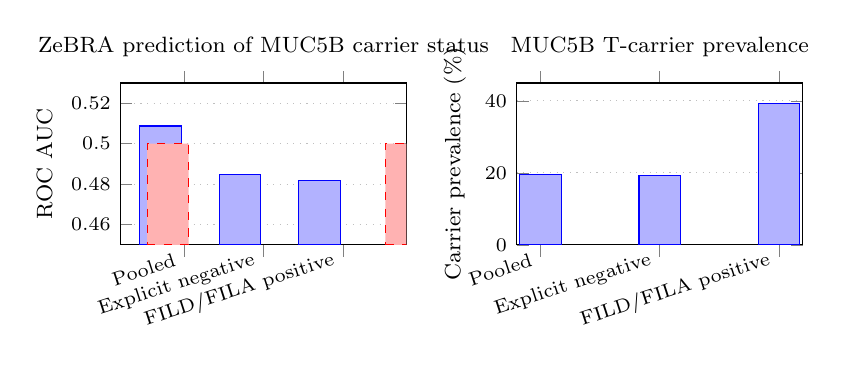
\begin{tikzpicture}
\begin{groupplot}[
group style={group size=2 by 1,horizontal sep=1.4cm},
width=0.43\textwidth,height=0.30\textwidth,
tick label style={font=\scriptsize},label style={font=\footnotesize},title style={font=\footnotesize},
ymajorgrids=true,major grid style={dotted}]
\nextgroupplot[
title={ZeBRA prediction of MUC5B carrier status},
ybar,bar width=15pt,ymin=0.45,ymax=0.53,
ylabel={ROC AUC},xtick={1,2,3},xticklabels={Pooled,Explicit negative,FILD/FILA positive},xticklabel style={font=\scriptsize,rotate=18,anchor=east}]
\addplot coordinates {(1,0.50875) (2,0.48471) (3,0.48168)};
\addplot+[no marks,dashed] coordinates {(0.5,0.5) (3.5,0.5)};
\nextgroupplot[
title={MUC5B T-carrier prevalence},
ybar,bar width=15pt,ymin=0,ymax=45,
ylabel={Carrier prevalence (\%)},xtick={1,2,3},xticklabels={Pooled,Explicit negative,FILD/FILA positive},xticklabel style={font=\scriptsize,rotate=18,anchor=east}]
\addplot coordinates {(1,19.58) (2,19.17) (3,39.29)};
\end{groupplot}
\end{tikzpicture}
\caption{ZeBRA does not reconstruct \textit{MUC5B} genotype. Left: ZeBRA discrimination of rs35705950 T-carrier status is at chance in the pooled cohort and within disease strata. Right: \textit{MUC5B} carrier prevalence is substantially higher among FILD/FILA-positive subjects, explaining how pooled disease-risk enrichment can arise without genotype reconstruction.}
\label{fig:muc5b-strata}
\end{figure*}

\subsection{Residual genomic information is localized in ZeBRA score space}

The absence of global incremental AUC does not imply zero conditional genomic information everywhere. We evaluated FILD/FILA prediction within bands defined by ZeBRA thresholds corresponding to control-FPR ranges. The residual contribution of \textit{MUC5B} is highly heterogeneous. In the 5--10\% FPR band, for example, the likelihood-ratio statistic for adding \textit{MUC5B} after ZeBRA was 16.55 ($p=4.74\times10^{-5}$); local AUC was 0.677 for \textit{MUC5B} versus 0.367 for ZeBRA. Conditional genomic information was also detected in the 2--5\%, 10--20\%, and 20--40\% bands (Fig.~\ref{fig:localized-rescue}, left).

These results provide the empirical bridge to Theorem~\ref{thm:main}: the relevant question is not whether genomics improves a population-wide ranking, but whether residual genomic likelihood evidence is strong enough to change a decision for patients whose clinical evidence lies near a chosen operating boundary.

\subsection{Boundary-targeted \textit{MUC5B} use improves matched-FPR sensitivity}

We therefore evaluated a clinically interpretable two-threshold rule. Patients above a stringent upper ZeBRA threshold are classified directly by ZeBRA. Patients below a lower threshold remain negative. Only patients between the two thresholds are eligible for \textit{MUC5B}-based rescue. Thresholds are estimated from the training split, and the resulting rule is evaluated on held-out subjects. A ZeBRA-only threshold is then selected to match the realized FPR of the rescue rule.

Across 100 repeated splits, the boundary rule increased sensitivity at essentially matched overall FPR. With an upper threshold corresponding to 0.5\% training-control FPR and a lower threshold corresponding to 10\%, mean sensitivity increased from 0.3587 for matched-FPR ZeBRA to 0.4033 with \textit{MUC5B} rescue ($\Delta=+0.0446$), while mean FPR was 0.02335 versus 0.02310. Mean LR$+$ increased from 15.58 to 17.54 and mean LR$-$ decreased from 0.657 to 0.611. The sensitivity advantage was positive in 97\% of the 100 repeated splits. The pattern across all evaluated threshold pairs is shown in Fig.~\ref{fig:localized-rescue} (right), with selected operating points in Table~\ref{tab:boundary-selected}.

\begin{figure*}[!t]
\centering
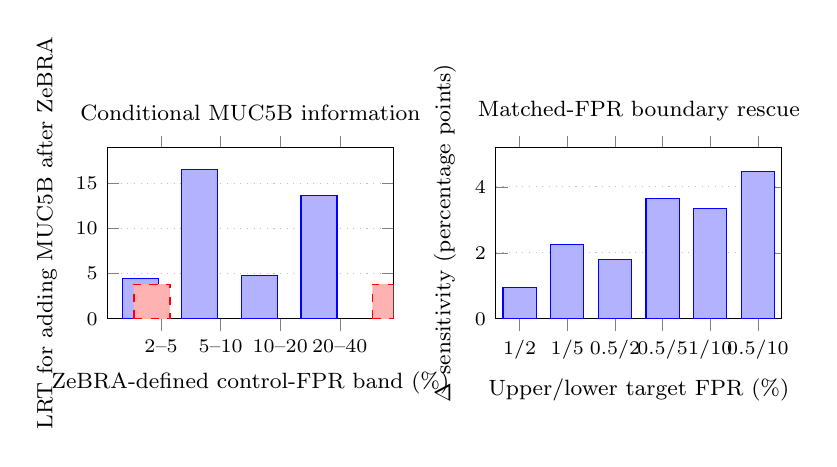
\begin{tikzpicture}
\begin{groupplot}[
group style={group size=2 by 1,horizontal sep=1.3cm},
width=0.43\textwidth,height=0.31\textwidth,
tick label style={font=\scriptsize},label style={font=\footnotesize},title style={font=\footnotesize},
ymajorgrids=true,major grid style={dotted}]
\nextgroupplot[
title={Conditional MUC5B information},
ybar,bar width=13pt,ymin=0,ymax=19,
ylabel={LRT for adding MUC5B after ZeBRA},
xtick={1,2,3,4},xticklabels={2--5,5--10,10--20,20--40},xlabel={ZeBRA-defined control-FPR band (\%)}]
\addplot coordinates {(1,4.44) (2,16.55) (3,4.77) (4,13.69)};
\addplot+[no marks,dashed] coordinates {(0.5,3.84) (4.5,3.84)};
\nextgroupplot[
title={Matched-FPR boundary rescue},
ybar,bar width=12pt,ymin=0,ymax=5.2,
ylabel={$\Delta$ sensitivity (percentage points)},
xtick={1,2,3,4,5,6},xticklabels={1/2,1/5,0.5/2,0.5/5,1/10,0.5/10},xlabel={Upper/lower target FPR (\%)}]
\addplot coordinates {(1,0.96) (2,2.25) (3,1.81) (4,3.66) (5,3.35) (6,4.46)};
\end{groupplot}
\end{tikzpicture}
\caption{Localized genomic utility. Left: conditional \textit{MUC5B} likelihood-ratio statistics vary strongly across ZeBRA score regions; the dashed line marks the nominal $\chi^2_1=3.84$ reference. Right: using \textit{MUC5B} only within a two-threshold ZeBRA decision band increases held-out sensitivity at essentially matched overall FPR.}
\label{fig:localized-rescue}
\end{figure*}

\begin{table*}[!t]
\caption{Selected matched-FPR boundary-rescue results over 100 repeated splits.}
\label{tab:boundary-selected}
\centering
\footnotesize
\setlength{\tabcolsep}{6pt}
\begin{tabular}{lrrrrrr}
\toprule
Upper/lower target FPR & ZeBRA sensitivity & Rescue sensitivity & $\Delta$ sensitivity & ZeBRA FPR & Rescue FPR & Rescue LR$+$\\
\midrule
1\% / 5\% & 0.3303 & 0.3528 & +0.0225 & 0.01844 & 0.01826 & 19.52\\
0.5\% / 5\% & 0.3121 & 0.3487 & +0.0366 & 0.01404 & 0.01400 & 25.21\\
1\% / 10\% & 0.3740 & 0.4075 & +0.0335 & 0.02753 & 0.02735 & 14.95\\
0.5\% / 10\% & 0.3587 & 0.4033 & +0.0446 & 0.02335 & 0.02310 & 17.54\\
\bottomrule
\end{tabular}
\end{table*}

This result is stronger than asking whether a global combined model has higher AUC. It demonstrates that germline information can improve an operating decision precisely where the clinical score is ambiguous, while providing little or no benefit to the global ranking.

\subsection{ROC-envelope analysis as supporting geometry}

A separate five-fold out-of-fold analysis compared ZeBRA with an exploratory fixed-region \textit{MUC5B} hybrid and the upper convex hull of the union of their ROC points. Empirical/interpolated AUC was 0.8142 for ZeBRA and 0.8095 for the hybrid; the convex hull of the union had AUC 0.8260. This hull is not a third scalar classifier and should not be interpreted as a deployable model. Rather, it is a geometric diagnostic showing that the two channels attain different favorable operating regions. We therefore treat the ROC hull as supporting evidence for regime-dependent complementarity rather than as the primary performance result.

\subsection{Empirical interpretation and limitations}

Taken together, the analyses support four statements. First, a near-term longitudinal clinical-history score substantially outperforms the selected genomic panel as a global predictor. Second, explicitly paired regularized modeling provides essentially no global FILD/FILA AUC increment from adding the complete genomic panel to ZeBRA, and proper scoring rules do not improve. Third, this is not because ZeBRA reconstructs \textit{MUC5B} genotype: global genotype prediction is at chance, and the apparent pooled tail association disappears within disease strata. Fourth, residual \textit{MUC5B} information remains locally useful and can improve held-out sensitivity when applied selectively near a ZeBRA operating boundary at matched overall FPR.

Several limitations prevent stronger causal or universal claims. The genomic panel is selected rather than a complete externally weighted IPF polygenic score. The local bands and threshold pairs are evaluated in the same Colorado resource and require independent replication or prospective prespecification. Repeated train/test splits share subjects and therefore should not be treated as independent biological replicates; split-wise quantiles summarize robustness to data partitioning rather than classical independent-sample confidence intervals. Most importantly, the notebook target construction assigns missing adjudication fields to zero. Accordingly, overall FPR in the operational target should not be described as FPR among fully adjudicated controls until that endpoint definition is independently verified.
}

\newcommand{\supplementarymaterial}{%
\appendices

\origsection{Operational phenotype and genomic input}
\label{app:targets}
The three phenotype fields were read from \texttt{REPHENOTYPES FOR IC.csv}. The operational notebook geometry maps \texttt{Y/y} to 1 and \texttt{N/n} to 0, assigns missing target values to 0, and excludes observations without an available ZeBRA score. For analyses requiring called rs35705950 genotype, 12,766 subjects remained, including 252 notebook-defined FILD/FILA positives and 2,499 \textit{MUC5B} T-allele carriers. Among stored phenotype records, 360 subjects were explicitly adjudicated FILD/FILA negative.

The processed genomic matrix was constructed by matching an expanded ILD/IPF candidate-locus list against the Colorado genomic header and taking the union with the pre-existing biological-driver panel. The expanded \texttt{MORE\_LOCI.csv} file contained 3,113 candidate records, of which 148 genotype columns were matched before union and de-duplication. The processed analysis matrix contains 171 distinct variant loci represented by one-hot genotype states. The reproducibility package treats \texttt{ILD\_TOP\_DRIVERS\_DATA.csv} as the processed genomic input and documents its schema in \texttt{zebra\_comp/README.md}.

\origsection{Full paired incremental-AUC summary}
\begin{table*}[!t]
\caption{Paired effect of adding the genomic panel to ZeBRA over 30 repeated splits.}
\centering
\footnotesize
\setlength{\tabcolsep}{8pt}
\begin{tabular}{lrrr}
\toprule
Target & Mean $\Delta$AUC & Median $\Delta$AUC & 2.5--97.5\% range\\
\midrule
FILD/FILA & +0.00043 & 0.00000 & $[-0.00507,\ 0.00408]$\\
Nonfibrotic ILD & -0.10052 & -0.08615 & $[-0.22577,\ -0.00506]$\\
Nonfibrotic ILA & -0.03737 & -0.03667 & $[-0.07384,\ -0.00705]$\\
\bottomrule
\end{tabular}
\end{table*}

\origsection{Local-information details}
\begin{table*}[!t]
\caption{Local FILD/FILA information within ZeBRA-defined control-FPR bands.}
\centering
\scriptsize
\setlength{\tabcolsep}{6pt}
\begin{tabular}{lrrrrrr}
\toprule
Band & $N$ & Cases & LRT $G\mid Z$ & $p$ & AUC ZeBRA & AUC \textit{MUC5B}\\
\midrule
2--5\% & 401 & 26 & 4.44 & 0.0352 & 0.577 & 0.595\\
5--10\% & 652 & 26 & 16.55 & $4.74\times10^{-5}$ & 0.367 & 0.677\\
10--20\% & 1,281 & 30 & 4.77 & 0.0289 & 0.558 & 0.586\\
20--40\% & 2,540 & 37 & 13.69 & $2.15\times10^{-4}$ & 0.516 & 0.635\\
\bottomrule
\end{tabular}
\end{table*}

\origsection{Full matched-FPR boundary-rescue summary}
\begin{table*}[!t]
\caption{Matched-FPR boundary rescue over 100 repeated splits. ``Upper/lower'' are training-control target FPRs defining the ZeBRA decision band.}
\centering
\scriptsize
\setlength{\tabcolsep}{5pt}
\begin{tabular}{lrrrrrrr}
\toprule
Upper/lower & ZeBRA sens. & Rescue sens. & $\Delta$ sens. & ZeBRA FPR & Rescue FPR & ZeBRA LR$+$ & Rescue LR$+$\\
\midrule
1\% / 2\% & 0.3046 & 0.3142 & +0.0096 & 0.01227 & 0.01228 & 25.43 & 26.03\\
1\% / 5\% & 0.3303 & 0.3528 & +0.0225 & 0.01844 & 0.01826 & 18.19 & 19.52\\
0.5\% / 2\% & 0.2919 & 0.3101 & +0.0181 & 0.00801 & 0.00802 & 38.16 & 39.67\\
0.5\% / 5\% & 0.3121 & 0.3487 & +0.0366 & 0.01404 & 0.01400 & 22.74 & 25.21\\
1\% / 10\% & 0.3740 & 0.4075 & +0.0335 & 0.02753 & 0.02735 & 13.75 & 14.95\\
0.5\% / 10\% & 0.3587 & 0.4033 & +0.0446 & 0.02335 & 0.02310 & 15.58 & 17.54\\
\bottomrule
\end{tabular}
\end{table*}
}

\begin{document}
\let\origsection\section
\renewcommand{\section}[1]{%
  \ifstrequal{#1}{Latent-state and information-channel formulation}{\empiricalcallout}{}%
  \ifstrequal{#1}{Scope and limitations}{\empiricalsection}{}%
  \origsection{#1}%
}
\let\origthebibliography\thebibliography
\renewcommand{\thebibliography}[1]{\supplementarymaterial\origthebibliography{#1}}
\documentclass[journal]{IEEEtran}

\usepackage{amsmath,amssymb,amsthm}
\usepackage{booktabs}
\usepackage{cite}
\usepackage{url}
\usepackage[hidelinks]{hyperref}
\usepackage{microtype}

\newtheorem{theorem}{Theorem}
\newtheorem{corollary}{Corollary}
\newtheorem{proposition}{Proposition}
\newtheorem{remark}{Remark}

\newcommand{\Pone}{\mathbb{P}_1}
\newcommand{\Pzero}{\mathbb{P}_0}
\newcommand{\Eone}{\mathbb{E}_1}
\newcommand{\Ezero}{\mathbb{E}_0}
\newcommand{\LR}{\Lambda}
\newcommand{\ind}{\mathbf{1}}

\title{Boundary-Localized Genomic Utility and Clinical-Tail Dominance:\\
A Likelihood-Ratio Theory for ZeBRA and Fibrotic Interstitial Lung Disease}

\author{Ishanu Chattopadhyay\\
Division of Biomedical Informatics, University of Kentucky College of Medicine}

\begin{document}
\maketitle

\begin{abstract}
Genomic risk and longitudinal clinical history provide distinct information channels for predicting future disease. We study when a static genomic channel can add predictive value once a clinical-history predictor has become strongly informative. In a Colorado fibrotic interstitial lung disease (ILD) analysis, ZeBRA---a longitudinal EHR-derived risk score---substantially outperformed a selected genomic panel in repeated held-out splits. A nonlinear global combination did not improve discrimination, and a separate paired regularized analysis found essentially zero global incremental FILD/FILA AUC from adding the complete genomic panel to ZeBRA (mean $\Delta$AUC $\approx4\times10^{-4}$). ZeBRA also predicted \textit{MUC5B} rs35705950 carrier status at chance level, excluding simple genotype reconstruction as an explanation. Nevertheless, \textit{MUC5B} retained significant conditional disease information in restricted ZeBRA-score regions, and a two-threshold genomic rescue rule increased held-out sensitivity by up to approximately 4.5 percentage points at essentially matched false-positive rate. We show that this pattern follows from a general likelihood-ratio argument. If residual genomic likelihood ratios are uniformly bounded while longitudinal clinical evidence can develop an extended likelihood-ratio tail, then genomic information can alter a likelihood-ratio decision only in a bounded neighborhood of the clinical decision threshold. Moreover, at sufficiently extreme specificity, the clinical likelihood-ratio test strictly dominates every genomic-only rule. The result explains how genomics can remain biologically and locally decision-relevant while contributing little to global near-term discrimination once clinical evidence becomes sufficiently strong.
\end{abstract}

\begin{IEEEkeywords}
ZeBRA, fibrotic interstitial lung disease, idiopathic pulmonary fibrosis, MUC5B, genomics, likelihood ratio, Neyman--Pearson lemma, Bayesian inference, decision boundary.
\end{IEEEkeywords}

\section{Motivating problem: ZeBRA and genomic risk in fibrotic ILD}

Fibrotic ILDs, including idiopathic pulmonary fibrosis (IPF), have a strong but non-Mendelian genetic component. The \textit{MUC5B} promoter variant rs35705950 is among the strongest common genetic risk factors for pulmonary fibrosis \cite{Seibold2011,Fingerlin2013,Allen2020}. At the same time, disease emergence is accompanied by an evolving sequence of clinically observable diagnoses, prescriptions, procedures, and comorbidities. ZeBRA is designed to summarize such routinely observed longitudinal clinical histories into a future-risk score without requiring laboratory tests, imaging, or questionnaires \cite{Onishchenko2026}.

The empirical question is not whether genomics is biologically important, but whether it supplies \emph{incremental predictive information} once a sufficiently informative near-term clinical-history score is already available. In 30 repeated held-out splits of the current Colorado FILD/FILA operational endpoint, mean AUC was approximately 0.814 for ZeBRA, 0.566 for the selected genomic panel, and 0.799 for a nonlinear combined model. Because overlapping repeated-split AUC distributions do not by themselves establish absence of incremental information, we separately performed a paired regularized analysis in which ZeBRA-only and ZeBRA-plus-genomics models were evaluated on the same held-out subjects. For FILD/FILA, the mean paired AUC increment was only $+0.00043$, the median increment was 0, and the 2.5th--97.5th percentile split-wise range spanned approximately $-0.0051$ to $+0.0041$; Brier score and log loss worsened in every split after adding the full genomic panel.

The absence of global gain is not explained by ZeBRA reconstructing the major genetic signal. Among subjects with called rs35705950 genotype, ZeBRA predicted \textit{MUC5B} carrier status at essentially chance level (AUC $\approx0.509$). A weak pooled enrichment of carriers in the extreme ZeBRA tail disappeared after stratification by FILD/FILA status, indicating that the pooled association is consistent with both predictors tracking disease rather than with clinical history encoding genotype. Yet \textit{MUC5B} remained conditionally informative within restricted ZeBRA operating regions. In the ZeBRA band corresponding approximately to 5--10\% control FPR, for example, adding \textit{MUC5B} after ZeBRA produced a likelihood-ratio statistic of 16.55 ($p\approx4.7\times10^{-5}$). A two-threshold rule that consulted \textit{MUC5B} only between a stringent upper and lower ZeBRA threshold increased held-out sensitivity by approximately 4.5 percentage points in one evaluated configuration while preserving essentially the same overall FPR.

The empirical pattern is therefore not a simple competition between modalities:
\begin{quote}
A strong genomic risk factor can be biologically important and locally decision-relevant, while contributing almost nothing to global discrimination once a strong clinical-history predictor is available.
\end{quote}

This motivates a likelihood-ratio theory of \emph{regime-dependent complementarity}: genomic information should matter most where the clinical evidence is close enough to the operating threshold that bounded residual genomic evidence can still change the decision.

\section{Latent-state and information-channel formulation}

Let $B_t$ denote the latent biological state at time $t$, $G$ the germline genomic state, and $E_{0:t}$ the accumulated non-genetic exposure history. The biological state evolves under the influence of $G$ and $E_{0:t}$. For a fixed future horizon $h>0$, define the disease-risk functional
\begin{equation}
\rho_h(B_t)
=\mathbb{P}(T\le t+h\mid T>t,B_t),
\label{eq:rho}
\end{equation}
where $T$ is the disease-event time. The clinical event sequence $C_{0:t}$ is a noisy observation of the latent biological trajectory $B_{0:t}$. In the idealized Bayesian limit, a clinical-history predictor satisfies
\begin{equation}
Z_h(C_{0:t})
=\mathbb{P}(T\le t+h\mid C_{0:t})
=\int \rho_h(b)\,d\mathbb{P}(B_t=b\mid C_{0:t}).
\label{eq:zposterior}
\end{equation}
Thus ZeBRA need not reconstruct $B_t$ or $G$; it estimates a disease-relevant functional of the latent state from the clinical observation channel.

For the theorem it is enough to reduce the problem to binary prediction. Let
\begin{equation}
Y=\ind\{T\le t+h\}\in\{0,1\},
\end{equation}
and write $C$ for the available clinical history. The genomic channel $G$ and clinical channel $C$ are then placed on equal statistical footing through their disease-versus-control likelihood ratios.

\section{Likelihood-ratio representation}

Let $\Pone(\cdot)=\mathbb{P}(\cdot\mid Y=1)$ and $\Pzero(\cdot)=\mathbb{P}(\cdot\mid Y=0)$. Assume the relevant distributions admit densities with respect to common dominating measures. Define the clinical likelihood ratio
\begin{equation}
\LR_C(c)=\frac{p(c\mid Y=1)}{p(c\mid Y=0)},
\label{eq:clinicalLR}
\end{equation}
and the residual genomic likelihood ratio conditional on clinical history
\begin{equation}
\LR_{G\mid C}(g;c)
=\frac{p(g\mid Y=1,C=c)}{p(g\mid Y=0,C=c)}.
\label{eq:conditionalGLR}
\end{equation}
The full joint likelihood ratio is
\begin{equation}
\LR_{C,G}(c,g)
=\frac{p(c,g\mid Y=1)}{p(c,g\mid Y=0)}.
\end{equation}
By the probability chain rule,
\begin{equation}
\boxed{
\LR_{C,G}(c,g)
=\LR_C(c)\,\LR_{G\mid C}(g;c).
}
\label{eq:factorization}
\end{equation}
No conditional-independence assumption is required.

If $Z$ is a calibrated clinical posterior, $Z=\mathbb{P}(Y=1\mid C)$, and $\pi=\mathbb{P}(Y=1)$, Bayes' rule yields
\begin{equation}
\frac{Z}{1-Z}
=\frac{\pi}{1-\pi}\LR_C(C),
\label{eq:zlr}
\end{equation}
so thresholding calibrated ZeBRA is equivalent to thresholding $\LR_C$. More generally, the same results apply whenever the clinical score is a strictly monotone transformation of $\LR_C$.

\section{Main theorem}

The theorem uses two explicit regularity assumptions.

\textbf{A1 (Uniformly bounded residual genomic evidence).} There exist constants $0<m\le 1\le M<\infty$ such that
\begin{equation}
0<m\le \LR_{G\mid C}(g;c)\le M<\infty
\label{eq:boundedconditional}
\end{equation}
for the relevant support of $(g,c)$, and the marginal genomic likelihood ratio
\begin{equation}
\LR_G(g)=\frac{p(g\mid Y=1)}{p(g\mid Y=0)}
\end{equation}
is bounded above by $M_G<\infty$. Non-Mendelian disease motivates finite genomic evidence, but does not by itself logically guarantee this uniform bound; A1 is therefore stated as an explicit regularity condition.

\textbf{A2 (Accumulating clinical evidence).} Clinical history is sequential, $C_n=(X_1,\ldots,X_n)$, and continued diagnoses, prescriptions, procedures, and comorbidities can produce an extended disease-evidence tail. Formally, $\LR_C$ is not bounded above on the relevant sequence of clinical histories: for arbitrarily large $K$ there are events with positive $\Pzero$ probability on which $\LR_C\ge K$.

\begin{theorem}[Boundary-localized genomic utility and clinical-tail dominance]
\label{thm:main}
Under A1--A2:

\emph{(i) Exact factorization.} The optimal joint disease-versus-control likelihood ratio is
\begin{equation}
\LR_{C,G}=\LR_C\LR_{G\mid C}.
\end{equation}

\emph{(ii) Boundary localization.} For any likelihood-ratio decision threshold $\lambda>0$, genomic information can change which side of the threshold an observation occupies only if
\begin{equation}
\boxed{
\frac{\lambda}{M}
\le \LR_C(c)
\le \frac{\lambda}{m}.
}
\label{eq:boundaryband}
\end{equation}
Equivalently,
\begin{equation}
\boxed{
-\log M
\le
\log \LR_C(c)-\log\lambda
\le
-\log m.
}
\label{eq:logboundaryband}
\end{equation}
Hence the genomic decision-relevant region has fixed width
\begin{equation}
\log(M/m)
\end{equation}
on the clinical log-likelihood scale, independent of where the decision boundary $\lambda$ is placed.

\emph{(iii) Genomic-only power is bounded.} For any test $\phi(G)\in[0,1]$ using genomics alone, with false-positive rate $\alpha=\Ezero[\phi(G)]$, its true-positive rate satisfies
\begin{equation}
\boxed{
\Eone[\phi(G)]\le M_G\alpha.
}
\label{eq:genomicpowerbound}
\end{equation}
Thus the positive likelihood ratio of any genomic-only decision rule is at most $M_G$.

\emph{(iv) Clinical superiority at extreme specificity.} For any $K>M_G$ with $\alpha_K=\Pzero(\LR_C\ge K)>0$, the clinical likelihood-ratio test
\begin{equation}
\phi_K(C)=\ind\{\LR_C(C)\ge K\}
\end{equation}
has
\begin{equation}
\frac{\Pone(\LR_C\ge K)}{\Pzero(\LR_C\ge K)}\ge K>M_G.
\label{eq:clinicalLRplus}
\end{equation}
Therefore, at the same FPR $\alpha_K$, its power is strictly greater than that of every genomic-only test. Moreover,
\begin{equation}
\alpha_K\le \frac{1}{K}\to0
\end{equation}
as $K\to\infty$. Hence the superiority occurs in the extreme-specificity limit.

\emph{(v) Clinical-tail dominance in the combined evidence.} Along sequences with $\LR_C\to\infty$,
\begin{equation}
\log \LR_{C,G}
=\log \LR_C+O(1),
\end{equation}
and therefore
\begin{equation}
\boxed{
\frac{\log\LR_{C,G}}{\log\LR_C}\to1.
}
\label{eq:taildominance}
\end{equation}
Thus bounded genomic evidence is asymptotically negligible relative to the accumulated clinical log-likelihood in the extreme clinical-evidence tail.
\end{theorem}

\begin{proof}
Part (i) is the chain rule:
\begin{align}
\LR_{C,G}(c,g)
&=\frac{p(c,g\mid Y=1)}{p(c,g\mid Y=0)}\\
&=\frac{p(c\mid Y=1)p(g\mid Y=1,c)}
        {p(c\mid Y=0)p(g\mid Y=0,c)}\\
&=\LR_C(c)\LR_{G\mid C}(g;c).
\end{align}

For part (ii), compare the clinical-only decision $\LR_C\ge\lambda$ with the joint decision $\LR_C\LR_{G\mid C}\ge\lambda$. If $\LR_C<\lambda/M$, then A1 gives $\LR_C\LR_{G\mid C}<\lambda$, so no genomic state can move the observation above threshold. Conversely, if $\LR_C>\lambda/m$, then $\LR_C\LR_{G\mid C}>\lambda$, so no genomic state can move the observation below threshold. Hence a threshold change is possible only on the interval in \eqref{eq:boundaryband}. Taking logarithms gives \eqref{eq:logboundaryband}, whose width is $\log(M/m)$ and does not depend on $\lambda$.

For part (iii), let $\phi(G)\in[0,1]$. Using the Radon--Nikodym identity under $\Pzero$,
\begin{align}
\Eone[\phi(G)]
&=\Ezero[\LR_G(G)\phi(G)]\\
&\le M_G\Ezero[\phi(G)]\\
&=M_G\alpha.
\end{align}
This proves \eqref{eq:genomicpowerbound} and holds for randomized as well as deterministic genomic rules.

For part (iv), define $A_K=\{c:\LR_C(c)\ge K\}$. Then
\begin{align}
\Pone(A_K)
&=\Ezero[\LR_C(C)\ind\{A_K\}]\\
&\ge K\Ezero[\ind\{A_K\}]\\
&=K\Pzero(A_K)\\
&=K\alpha_K.
\end{align}
Therefore the clinical rule has LR$+$ at least $K$. If $K>M_G$, any genomic-only test with the same FPR $\alpha_K$ has power at most $M_G\alpha_K<K\alpha_K\le\Pone(A_K)$. By the Neyman--Pearson lemma \cite{NeymanPearson1933}, thresholding $\LR_C$ is also the most powerful rule among all tests measurable with respect to $C$ at the corresponding size, with the usual boundary randomization if needed.

Finally, because $\Ezero[\LR_C]=1$, Markov's inequality gives
\begin{equation}
\alpha_K=\Pzero(\LR_C\ge K)\le\frac{1}{K},
\end{equation}
so $\alpha_K\to0$ as $K\to\infty$. For part (v), A1 implies $\log\LR_{G\mid C}=O(1)$, and therefore
\begin{equation}
\log\LR_{C,G}=\log\LR_C+O(1).
\end{equation}
Dividing by $\log\LR_C$ and letting $\LR_C\to\infty$ yields \eqref{eq:taildominance}.
\end{proof}

\begin{corollary}[Posterior-risk form for ZeBRA]
\label{cor:zebra}
If ZeBRA is calibrated so that $Z=\mathbb{P}(Y=1\mid C)$, let $\tau\in(0,1)$ be any ZeBRA decision threshold and define posterior-odds threshold $\kappa=\tau/(1-\tau)$. Then genomic information can change the decision only if
\begin{equation}
\boxed{
\frac{\kappa}{M}
\le
\frac{Z}{1-Z}
\le
\frac{\kappa}{m}.
}
\label{eq:zboundary}
\end{equation}
Equivalently,
\begin{equation}
-\log M
\le
\operatorname{logit}(Z)-\operatorname{logit}(\tau)
\le
-\log m.
\end{equation}
Thus genomic utility is localized around \emph{whatever} ZeBRA operating boundary is chosen.
\end{corollary}

\begin{proof}
Equation \eqref{eq:zlr} shows that ZeBRA posterior odds differ from $\LR_C$ by the positive constant prior odds $\pi/(1-\pi)$. Substitution into Theorem~\ref{thm:main}(ii) yields the result.
\end{proof}

\begin{corollary}[Any genomic model inherits the bound]
Let $S=f(G)$ be any measurable genomic predictor, including a polygenic risk score, gradient-boosted model, random forest, neural network, or generative genomic model. If the full genomic likelihood ratio is bounded, then the likelihood ratio of $S$ is also bounded. Therefore no deterministic compression or machine-learning transformation of the same genomic information can evade the finite-evidence and extreme-specificity conclusions of Theorem~\ref{thm:main}.
\end{corollary}

\begin{proof}
For a score value $s$, the score likelihood ratio can be written as a conditional average of the full genomic likelihood ratio under $\Pzero$:
\begin{equation}
\LR_S(s)=\mathbb{E}_0[\LR_G(G)\mid S=s].
\end{equation}
A conditional expectation of a random variable bounded above by $M_G$ is itself bounded above by $M_G$. The analogous lower bound follows if $\LR_G$ is bounded away from zero.
\end{proof}

\section{Why the clinical channel can have an extended tail}

The theorem does not assume that every later clinical event is informative, nor that disease becomes perfectly observable. It requires only that the clinical channel can accumulate sufficiently strong evidence on some disease trajectories. For a sequential history $C_n=(X_1,\ldots,X_n)$, the clinical likelihood ratio factorizes exactly as
\begin{equation}
\LR_C(C_n)
=\prod_{k=1}^{n}
\frac{p(X_k\mid Y=1,X_{<k})}
     {p(X_k\mid Y=0,X_{<k})},
\label{eq:sequentialLR}
\end{equation}
so that
\begin{equation}
\log\LR_C(C_n)
=\sum_{k=1}^{n}
\log
\frac{p(X_k\mid Y=1,X_{<k})}
     {p(X_k\mid Y=0,X_{<k})}.
\label{eq:sequentiallogLR}
\end{equation}
This is the standard likelihood-ratio accumulation underlying sequential testing \cite{Wald1945}. The germline genomic state does not acquire new variants as the disease approaches, whereas the clinical history can acquire additional diagnoses, procedures, prescriptions, and comorbidities. The difference is therefore not that clinical and genomic predictors obey different probability laws; both enter Bayes' rule as evidence. The difference is that one channel is static while the other is longitudinal and can supply repeated likelihood-ratio factors.

Equation \eqref{eq:sequentialLR} also clarifies the sense in which clinical odds may rise sharply: likelihood evidence adds in log space but multiplies in odds space. No claim of exponential growth follows from AUC alone. Rather, when a sequence contains repeated positive log-likelihood increments, posterior odds are the exponential of their accumulated sum.

\section{Interpretation of the ILD/IPF observations}

The theorem organizes the empirical findings into four statements.

\subsection{Global genomic augmentation can be negligible even when genomics is biologically important}
A strong clinical-history score can already order most case--control pairs correctly. Global AUC averages over the entire score distribution, whereas Theorem~\ref{thm:main}(ii) concerns whether residual genomic evidence can change a decision near a specified threshold. Thus a substantial local decision benefit can coexist with negligible global AUC change. This is precisely what the paired FILD/FILA analysis shows: adding the complete genomic panel changes mean AUC by only about $4\times10^{-4}$ while worsening Brier score and log loss.

The result should not be interpreted as a universal claim that EHR and genomic predictors are never complementary. Large biobank studies have reported additive value from combining EHR-derived and polygenic scores \cite{Detrois2025}. Our claim is regime-dependent: complementarity should depend on prediction horizon, clinical predictor strength, and the subject's location in clinical likelihood-ratio space. A static susceptibility score may add more to a weaker or longer-horizon clinical predictor than to a highly informative near-term trajectory score.

\subsection{Weak ZeBRA--genotype association is evidence for distinct channels, not genomic irrelevance}
ZeBRA predicts \textit{MUC5B} carrier status at chance level. The weak pooled enrichment observed only in the extreme ZeBRA tail disappears after conditioning on disease status, consistent with a common-cause explanation through FILD/FILA risk rather than genotype reconstruction. The relevant quantity for prediction is therefore not $I(Z;G)$ itself but the residual disease evidence supplied by $G$ at a particular clinical state, represented by $\LR_{G\mid C}$. A high-effect allele can be nearly unpredictable from ZeBRA globally yet still alter the posterior odds for boundary-adjacent patients.

\subsection{Local information and matched-FPR rescue instantiate boundary localization}
Within several ZeBRA-defined FPR bands, \textit{MUC5B} contributes significant information after conditioning on ZeBRA. A two-threshold rule that uses genotype only between a stringent upper threshold and a lower threshold converts that local information into an operating benefit. Across repeated held-out splits, sensitivity increases by up to approximately 4.5 percentage points at essentially unchanged overall FPR. This is the empirical quantity most directly aligned with Theorem~\ref{thm:main}(ii): genomic evidence changes decisions selectively in a clinical-score region rather than improving the population-wide ranking.

\subsection{Why ZeBRA should dominate at very high specificity}
For any genomic-only rule, Theorem~\ref{thm:main}(iii) bounds achievable LR$+$ by $M_G$. In contrast, a clinical likelihood-ratio tail above threshold $K$ has LR$+\ge K$, and its FPR is at most $1/K$. Therefore, once clinical history reaches likelihood-ratio levels larger than the maximum genomic Bayes factor, the clinical channel must be superior to every genomic-only predictor at those extreme-specificity operating points. The empirical observation that ZeBRA achieves large LR$+$ at stringent specificity is therefore more directly relevant to the theory than AUC alone.

The expected geometry is consequently a transition from inherited susceptibility, through a boundary region in which both channels can matter, to clinical-tail dominance. It is not a uniform competition between globally interchangeable predictors.

\section{Scope and limitations}

The theory is a statement about information channels, not about a particular machine-learning algorithm. It does not require independence between genomics and clinical history; dependence is retained explicitly through $\LR_{G\mid C}$. It also does not claim that genomics changes no posterior probabilities away from the boundary; it states that under A1 bounded genomic evidence cannot change the binary likelihood-ratio \emph{decision} sufficiently far from the boundary.

Five qualifications are important. First, A1 is a uniform boundedness assumption, not a consequence of the word ``non-Mendelian.'' Its empirical plausibility must be assessed for the genomic state under study. Second, high AUC alone does not imply an extended clinical likelihood-ratio tail; the relevant empirical evidence is high likelihood ratio at stringent specificity together with the sequential structure of the clinical record. Third, the Colorado genomic panel is a selected candidate panel rather than a complete externally weighted IPF polygenic risk score. Fourth, the local regions and threshold pairs are exploratory within the same resource and require prespecified or external replication. Repeated train/test splits share subjects and summarize robustness to partitioning; they are not independent biological replicates. Fifth, the current operational target construction assigns missing adjudication fields to 0. Overall false-positive rates therefore refer to that operational target and should not be equated with false-positive rates among explicitly adjudicated negatives without a separate ascertainment analysis.

The current data consequently support a narrow predictive claim rather than a causal one: broad genomic augmentation provides little global near-term gain conditional on a strong clinical-history score, while specific genomic information retains measurable local decision utility. Independent cohorts, stronger genomic comparators, additional diseases, and multiple prediction horizons are needed to establish the generality of the proposed regime transition.

\section{Conclusion}

Genomic susceptibility and longitudinal clinical history are distinct information channels whose incremental value need not be uniform across risk space. Bayes' rule factorizes their joint evidence into clinical and residual genomic likelihood-ratio factors. Under explicitly bounded residual genomic evidence, genomics can change a clinical decision only within a bounded neighborhood of the chosen clinical likelihood-ratio threshold. If clinical evidence can develop an extended upper tail, a sufficiently stringent clinical likelihood-ratio rule eventually dominates every bounded genomic-only rule.

The current fibrotic ILD results show the predicted qualitative geometry. ZeBRA is substantially stronger than the selected genomic panel globally; adding the full genomic panel produces essentially zero paired FILD/FILA AUC gain; ZeBRA does not reconstruct \textit{MUC5B} genotype; yet \textit{MUC5B} retains significant conditional disease information within restricted ZeBRA regions and improves matched-FPR sensitivity when applied selectively near a decision boundary. The appropriate conclusion is therefore not that genomics ceases to matter, but that \emph{genomic complementarity is a regime rather than a universal property}: as longitudinal clinical evidence becomes sufficiently informative, genomic utility contracts toward the clinical decision boundary.

\begin{thebibliography}{99}

\bibitem{Onishchenko2026}
D.~Onishchenko, J.~A. Mastrianni, and I.~Chattopadhyay,
``Passive early screening for Alzheimer's disease and related dementias using EHR comorbidity patterns,''
\emph{npj Digital Medicine}, vol.~9, 2026, doi: 10.1038/s41746-026-02954-2.

\bibitem{Seibold2011}
M.~A. Seibold \emph{et al.},
``A common \textit{MUC5B} promoter polymorphism and pulmonary fibrosis,''
\emph{New England Journal of Medicine}, vol.~364, no.~16, pp.~1503--1512, 2011, doi: 10.1056/NEJMoa1013660.

\bibitem{Fingerlin2013}
T.~E. Fingerlin \emph{et al.},
``Genome-wide association study identifies multiple susceptibility loci for pulmonary fibrosis,''
\emph{Nature Genetics}, vol.~45, no.~6, pp.~613--620, 2013, doi: 10.1038/ng.2609.

\bibitem{Allen2020}
R.~J. Allen \emph{et al.},
``Genome-wide association study of susceptibility to idiopathic pulmonary fibrosis,''
\emph{American Journal of Respiratory and Critical Care Medicine}, vol.~201, no.~5, pp.~564--574, 2020, doi: 10.1164/rccm.201905-1017OC.

\bibitem{Detrois2025}
K.~E. Detrois, T.~Hartonen, M.~Teder-Laving, \emph{et al.},
``Cross-biobank generalizability and accuracy of electronic health record-based predictors compared to polygenic scores,''
\emph{Nature Genetics}, vol.~57, pp.~2136--2145, 2025, doi: 10.1038/s41588-025-02298-9.

\bibitem{NeymanPearson1933}
J.~Neyman and E.~S. Pearson,
``On the problem of the most efficient tests of statistical hypotheses,''
\emph{Philosophical Transactions of the Royal Society of London. Series A}, vol.~231, pp.~289--337, 1933, doi: 10.1098/rsta.1933.0009.

\bibitem{Wald1945}
A.~Wald,
``Sequential tests of statistical hypotheses,''
\emph{The Annals of Mathematical Statistics}, vol.~16, no.~2, pp.~117--186, 1945.

\bibitem{CoverThomas2006}
T.~M. Cover and J.~A. Thomas,
\emph{Elements of Information Theory}, 2nd~ed.
Hoboken, NJ, USA: Wiley, 2006.

\end{thebibliography}

\end{document}

\end{document}
